% ===========================================================================
\section{A geometria exata do reticulado}\label{sec:geometria}
% ===========================================================================

Nesta seção $k\ge2$, $\Seed_k$ é a semente da Definição~\ref{def:bloco} e
$\rB=\rB_{\Seed_k}$ é a distância relativa da Definição~\ref{def:rho}. O objetivo
é calcular $\rB$ exatamente nos primos de $A_k$.

\subsection{A distância ao inteiro mais próximo}

O reticulado $\Lat(\Seed_k)$ é, por construção, um subconjunto dos logaritmos de
inteiros maiores que $1$. Isso dá imediatamente uma cota inferior para qualquer
distância a ele: a distância ao inteiro mais próximo. O lema seguinte calcula essa
distância.

\begin{lema}[vizinho inteiro]\label{lema:vizinho}
Sejam $q,m$ inteiros com $q\ge2$, $m\ge2$ e $m\neq q$. Então
\[
  \bigl|\nfreq q-\nfreq m\bigr| \;\ge\; \log\!\Bigl(1+\frac1q\Bigr).
\]
Além disso, a igualdade é atingida em $m=q+1$.
\end{lema}

\begin{proof}
Se $m>q$, então $m\ge q+1$ e a monotonicidade de $\log$ dá
$\nfreq m-\nfreq q\ge\log(q+1)-\log q=\log(1+1/q)$.

Se $m<q$, então $m\le q-1$ e
\[
  \nfreq q-\nfreq m \;\ge\; \log q-\log(q-1) \;=\; \log\frac{q}{q-1}.
\]
Basta comparar os dois candidatos: $\frac{q}{q-1}\ge\frac{q+1}{q}$ porque
$q^2\ge (q-1)(q+1)=q^2-1$. Logo $\log\frac{q}{q-1}\ge\log(1+1/q)$, e a cota vale
nos dois casos.
\end{proof}

O Lema~\ref{lema:vizinho} é a peça central de tudo o que segue, e sua leitura
geométrica é simples: entre todos os logaritmos de inteiros, o mais próximo de
$\nfreq q$ é sempre $\nfreq{q+1}$, e a distância vale $\approx 1/q$. Nenhum
conjunto de geradores pode fazer melhor do que isso, porque o reticulado que eles
geram está contido nesse conjunto.

\subsection{Uma cota uniforme sobre o bloco}

\begin{teorema}\label{teo:cota}
Seja $k\ge1$ e $q\in\Pi_k$. Então
\[
  \rB(q) \;\ge\; \frac{1}{2^{k+1}\,(k+1)\,\log 2}.
\]
\end{teorema}

\begin{proof}
Pelo Lema~\ref{lema:vizinho} e pela definição de $\rB$,
\[
  \rB(q) \;\ge\; \frac{\log(1+1/q)}{\log q}.
\]
Usamos duas desigualdades elementares. Primeiro, $\log(1+x)\ge \frac{x}{1+x}$ para
$x>0$; com $x=1/q$ obtemos $\log(1+1/q)\ge \frac{1}{q+1}$. Segundo, como
$q<2^{k+1}$, temos $q+1\le 2^{k+1}$ e portanto
\[
  \frac{1}{q+1}\;\ge\;\frac{1}{2^{k+1}} .
\]
Finalmente $\log q<\log 2^{k+1}=(k+1)\log 2$. Combinando,
\[
  \rB(q)\;\ge\;\frac{1/(q+1)}{\log q}\;\ge\;
  \frac{2^{-(k+1)}}{(k+1)\log 2}
  \;=\;\frac{1}{2^{k+1}(k+1)\log 2}. \qedhere
\]
\end{proof}

\subsection{O valor exato}

A cota do Teorema~\ref{teo:cota} é atingida, e por um motivo que vale enunciar
separadamente: o vizinho de um primo ímpar está sempre no reticulado.

\begin{lema}\label{lema:qmaisum}
Seja $k\ge2$ e $q\in\Pi_k$. Então todo fator primo de $q+1$ é menor que $2^k$; em
outras palavras, $q+1$ é $\Seed_k$-suave.
\end{lema}

\begin{proof}
Como $q\ge3$ é ímpar, $q+1$ é par e maior que $2$, logo não é primo. Seja $r$ um
fator primo de $q+1$. Se $r=2$, então $r<2^k$ porque $k\ge2$. Se $r$ é ímpar,
escreva $q+1=rs$; como $q+1$ é par e $r$ é ímpar, $s$ é par, logo $s\ge2$ e
\[
  r\;\le\;\frac{q+1}{2}\;\le\;\frac{2^{k+1}}{2}\;=\;2^k .
\]
Sendo $r$ ímpar e $2^k$ par, segue $r<2^k$.
\end{proof}

\begin{teorema}[valor exato]\label{teo:exato}
Seja $k\ge2$ e $q\in\Pi_k$. Então
\[
  \rB(q) \;=\; \frac{\log\bigl(1+1/q\bigr)}{\log q} .
\]
\end{teorema}

\begin{proof}
A desigualdade $\ge$ é o Lema~\ref{lema:vizinho}, pois todo elemento de
$\Lat(\Seed_k)$ é o logaritmo de um inteiro maior que $1$, e esse inteiro não é
$q$ (o reticulado é gerado por primos menores que $q$).

Para $\le$, o Lema~\ref{lema:qmaisum} diz que $q+1=\prod_{p\in\Seed_k}p^{e_p}$,
logo $\nfreq{q+1}=\sum e_p\nfreq p\in\Lat(\Seed_k)$. Como
\[
  \bigl|\nfreq q-\nfreq{q+1}\bigr| = \log\Bigl(1+\frac1q\Bigr),
\]
o mínimo que define $\rB(q)$ não excede esse valor.
\end{proof}

O Teorema~\ref{teo:exato} é o resultado central do artigo, e a sua demonstração
tem duas linhas de conteúdo: a distância não pode ser menor que a distância ao
inteiro mais próximo, e o inteiro mais próximo está sempre disponível. O
reticulado gerado pelos primos de um bloco é, na escala $1/q$, exatamente tão fino
quanto o conjunto de todos os logaritmos de inteiros. Não há como escolher uma
base melhor.

\subsection{O mínimo sobre o bloco}

\begin{definicao}\label{def:g}
Para $q\ge2$ seja
\[
  g(q) \;=\; \frac{\log(1+1/q)}{\log q}, \qquad q_k=\max\Pi_k .
\]
\end{definicao}

\begin{corolario}\label{cor:min}
Para $k\ge2$, $\rB_{\min}(k)=\min_{q\in\Pi_k}\rB(q)$ é atingido em $q_k$ e vale
\[
  \rB_{\min}(k) \;=\; g(q_k) \;=\; \frac{\log(1+1/q_k)}{\log q_k}.
\]
\end{corolario}

\begin{proof}
Pelo Teorema~\ref{teo:exato}, $\rB(q)=g(q)$ em $\Pi_k$. A função $g$ é estritamente
decrescente em $[2,\infty)$: o numerador $\log(1+1/q)$ decresce e o denominador
$\log q$ cresce, ambos positivos. Logo o mínimo de $g$ sobre $\Pi_k$ é $g(q_k)$.
\end{proof}

\begin{corolario}\label{cor:assint}
Para $k\ge2$,
\[
  \frac{1}{2^{k+1}(k+1)\log 2} \;\le\; \rB_{\min}(k) \;\le\;
  \frac{1}{q_k\log q_k}\Bigl(1+O\bigl(q_k^{-1}\bigr)\Bigr),
\]
e portanto $\rB_{\min}(k)\asymp 1/(q_k\log q_k)$, isto é,
$\rB_{\min}(k)=\Theta\bigl(2^{-k}/k\bigr)$.
\end{corolario}

\begin{proof}
A cota inferior é o Teorema~\ref{teo:cota}. Para a superior, use
$\log(1+x)\le x$: $g(q_k)\le 1/(q_k\log q_k)$. Como
$2^k\le q_k<2^{k+1}$, tem-se $q_k\asymp 2^k$ e $\log q_k\asymp k$.
\end{proof}

A Tabela~\ref{tab:rho} compara o valor exato com a cota. A convergência é rápida:
a razão entre os dois é $1{,}03$ já em $k=4$ e $1{,}000$ em $k=16$.

\begin{table}[htbp]
\centering
\small
\begin{tabular}{rrrrr}
\toprule
$k$ & $q_k$ & $\rB_{\min}(k)$ & $\bigl(2^{k+1}(k+1)\log 2\bigr)^{-1}$ & razão \\
\midrule
4  & $31$      & $9{,}245\times10^{-3}$ & $9{,}017\times10^{-3}$ & 1,025 \\
6  & $127$     & $1{,}619\times10^{-3}$ & $1{,}610\times10^{-3}$ & 1,006 \\
8  & $509$     & $3{,}149\times10^{-4}$ & $3{,}131\times10^{-4}$ & 1,006 \\
10 & $2\,039$  & $6{,}434\times10^{-5}$ & $6{,}404\times10^{-5}$ & 1,005 \\
12 & $8\,191$  & $1{,}355\times10^{-5}$ & $1{,}355\times10^{-5}$ & 1,000 \\
14 & $32\,749$ & $2{,}937\times10^{-6}$ & $2{,}935\times10^{-6}$ & 1,001 \\
16 & $131\,071$& $6{,}475\times10^{-7}$ & $6{,}475\times10^{-7}$ & 1,000 \\
\bottomrule
\end{tabular}
\caption{O mínimo de $\rB$ sobre o bloco e a cota do Teorema~\ref{teo:cota}.}
\label{tab:rho}
\end{table}

\begin{figure}[htbp]
\centering
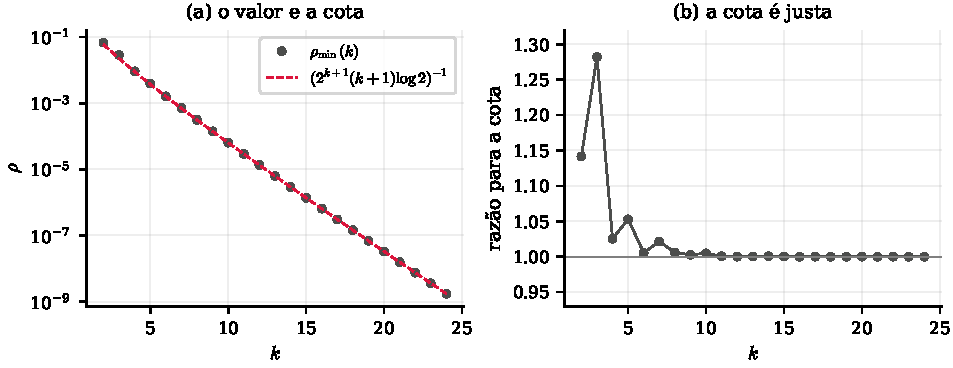
\includegraphics[width=0.95\textwidth]{figuras/f4_reticulado.pdf}
\caption{(a) $\rB_{\min}(k)$ e a cota do Teorema~\ref{teo:cota}, em escala
logarítmica. (b) A razão entre os dois; as oscilações nos blocos pequenos são os
saltos de $q_k$ quando o topo do bloco deixa de ser primo.}
\label{fig:reticulado}
\end{figure}

\subsection{O reticulado separa, e a margem é exata}

Juntando o Teorema~\ref{teo:exato} com o Corolário~\ref{cor:zero} obtém-se a
descrição completa da função $\rB$ sobre um bloco.

\begin{corolario}[os dois valores de $\rB$]\label{cor:doisvalores}
Seja $k\ge2$. Para $m\in A_k$:
\[
  \rB(m) \;=\;
  \begin{cases}
    0, & \text{se } m \text{ é composto},\\[2pt]
    g(m), & \text{se } m \text{ é primo}.
  \end{cases}
\]
Em particular, para todo $\theta$ com $0<\theta<\rB_{\min}(k)$,
\[
  \{m\in A_k : \rB(m) > \theta\} \;=\; \Pi_k .
\]
\end{corolario}

\begin{proof}
Se $m$ é composto, o Lema~\ref{lema:bloco} garante que todos os seus fatores
primos estão em $\Seed_k$, logo $m$ é $\Seed_k$-suave e
$\rB(m)=0$ pelo Corolário~\ref{cor:zero}. Se $m$ é primo, o
Teorema~\ref{teo:exato} dá $\rB(m)=g(m)>0$. A segunda afirmação segue porque $g$
é positiva e $\rB_{\min}(k)$ é o seu mínimo sobre $\Pi_k$.
\end{proof}

A leitura do Corolário~\ref{cor:doisvalores} merece cuidado, porque é fácil
transformá-la em algo que ela não diz. O que ele afirma é que a separação é
\emph{perfeita e com margem}: os compostos dão exatamente zero e os primos dão no
mínimo $\rB_{\min}(k)$. Todo limiar $\theta$ estritamente entre esses dois níveis
classifica corretamente o bloco inteiro. A margem, isto é, a distância entre os
dois níveis, vale exatamente
\[
  \rB_{\min}(k) \;=\; \frac{\log(1+1/q_k)}{\log q_k} \;\sim\; \frac{1}{q_k\log q_k},
\]
e é essa quantidade — e não outra — que mede a resolução com que a geometria
logarítmica distingue um primo de um composto. Ela decai como $1/(q\log q)$ com o
tamanho do primo, o que é o preço intrínseco da representação.

Não há, portanto, um \emph{gradiente} de primalidade: fora do conjunto dos primos,
$\rB$ é identicamente nulo sobre o bloco. Um inteiro composto de $A_k$ não está
``quase'' no reticulado — está nele, exatamente, e a distância zero é o conteúdo
aritmético do Lema~\ref{lema:bloco} traduzido para a reta.

\subsection{Por que a rota diofantina é desnecessária}

A cota do Teorema~\ref{teo:cota} poderia, em princípio, ser obtida pela teoria de
formas lineares em logaritmos, que fornece minorantes para
$\bigl|\sum e_i\nfreq{p_i}-\nfreq m\bigr|$ quando $m$ não é o produto
correspondente \cite{baker}. Essas cotas são da ordem de
$\exp\bigl(-C\,k\log^2 2\log k\bigr)$ — duplamente exponenciais em $k$ —, e para
$k=16$ ficam dezenas de ordens de grandeza abaixo do valor real.

A razão da discrepância é instrutiva. Os teoremas de formas lineares controlam o
\emph{pior caso} de uma combinação inteira arbitrária de logaritmos de primos.
Aqui o objeto não é arbitrário: queremos a distância de $\nfreq q$ ao conjunto dos
$\nfreq m$ com $m$ inteiro, e os inteiros são ordenados. A ordenação resolve o
problema: o vizinho é sempre $q+1$, e não há nada a estimar. Toda a dificuldade da
aproximação diofantina vem de permitir coeficientes negativos e geradores
arbitrários; a restrição ao reticulado dos inteiros elimina essa dificuldade.

Vale sublinhar o contraste, porque ele é o resumo matemático desta seção: o
problema \emph{geral} de aproximar logaritmos por combinações inteiras é profundo;
o problema \emph{restrito} que a aritmética formula é elementar. E é justamente a
restrição — o fato de o reticulado ser gerado pelos mesmos inteiros que se quer
classificar — que explica por que a irredutibilidade logarítmica, como problema de
aproximação, não carrega dificuldade diofantina alguma.
